\subsubsection{Model performance}
\label{sub:comb_performance}

The final section of this chapter presents results of experiments with multi-input
deep neural networks conducted in the scope of this work.
In the following paragraphs, classification and regression performance on all
data sets is listed and analyzed in detail.
The concluding results chapter (ch.~\ref{sec:res_summary}) will then put these
outcomes in relation to previously trained models.

\begin{table}
  \begin{tabular}{lrrrrrrr}
    \toprule
    & \multicolumn{4}{l}{Classification} & \multicolumn{3}{l}{Regression} \\
    \midrule
    Data set & CCE & Acc & Ret Acc & Fav Acc & MAE & Ret MAE & Fav MAE \\
    \midrule
    Celebrities & 0.80 & 65.16\% & 61.91\% & 68.40\% & 3,286.16 & 1,438.98 & 5,133.35 \\
    Politicians & 0.82 & 65.34\% & 64.22\% & 66.46\% & 447.61 & 262.78 & 632.44 \\
    Companies & 0.62 & 73.52\% & 75.88\% & 71.15\% & 19.41 & 10.99 & 27.84 \\
    Combined & 0.76 & 68.42\% & 70.05\% & 66.79\% & 401.52 & 201.70 & 601.33 \\
    \bottomrule
  \end{tabular}
  \caption{Summary of results for multi-input deep neural networks}
  \label{tab:deep2_results}
\end{table}

Table~\ref{tab:deep2_results} summarizes multi-input model results for both
engagement classification and regression.
As with all models in this work, metrics are calculated on held-out validation
examples.
Overall classification performance is similar for all data sets, as CCE loss values
even out between 0.62 and 0.82.
These results account for an overall classification accuracy, i.e., percentage
of correctly classified examples, of 65 to 75\%.
Best performance is achieved on the company data set, which is also the most
imbalanced data set when looking at class distributions (see ch.~\ref{sec:engagement_stats}).
In contrast to that, performance on the smaller celebrity and politician data sets
worsens.
Tweets from the larger, combined data sets are classified correctly 68\% of the
time.
Thus, classification performance seems not to be dependent on data set size alone.
Notable differences in retweet and favorite classification accuracy exist,
with the spread being widest for celebrity (6.49\%) and smallest for
politician tweets (2.24\%).
It has to be mentioned, that accuracies of more than 90\% were achievable on all
data sets when ignoring overfitting and solely focussing on training loss.
This once again points to the difficulty of learning generalizable models for
the complex task of engagement prediction.
As expected, MAE values for the regression task are of varying magnitude.
Predictions on more narrow engagement distributions (e.g., company data set)
are most precise than their counterparts on data sets containing many outliers
(e.g., celebrity data set).
As with classifications, notable differences between retweet and favorite prediction
can be identified.
In general, retweet predictions are most accurate, with favorite error values
being about three times bigger on all data sets.
According to the procudure applied in previous results chapters, both classification
and regression performance are analyzed in more detail in the following paragraphs.

\begin{figure}[h]
\begin{subfigure}{.5\textwidth}
  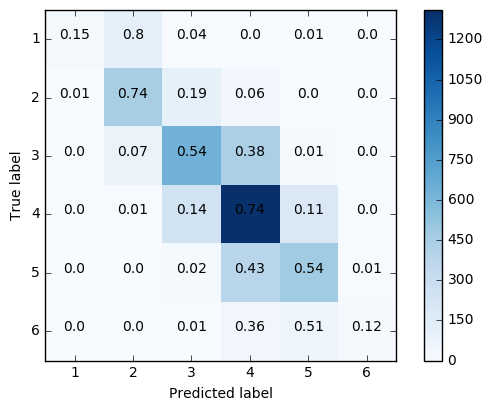
\includegraphics[width=.95\linewidth]{img/celeb_d2_cm_retweets}
  \caption{Celebrity data set}
  \label{fig:retw_distr_sub1}
\end{subfigure}%
\begin{subfigure}{.5\textwidth}
  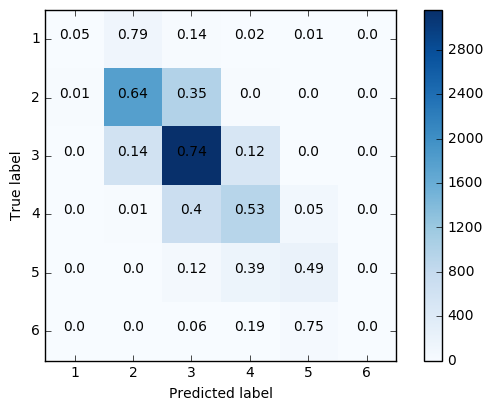
\includegraphics[width=.95\linewidth]{img/polit_d2_cm_retweets}
  \caption{Politician data set}
  \label{fig:retw_distr_sub2}
\end{subfigure}
\begin{subfigure}{.5\textwidth}
  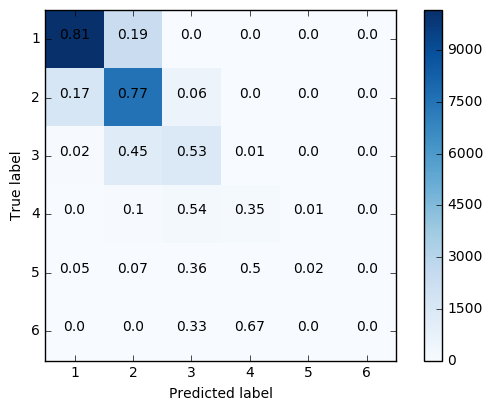
\includegraphics[width=.95\linewidth]{img/corp_d2_cm_retweets}
  \caption{Company data set}
  \label{fig:retw_distr_sub3}
\end{subfigure}%
\begin{subfigure}{.5\textwidth}
  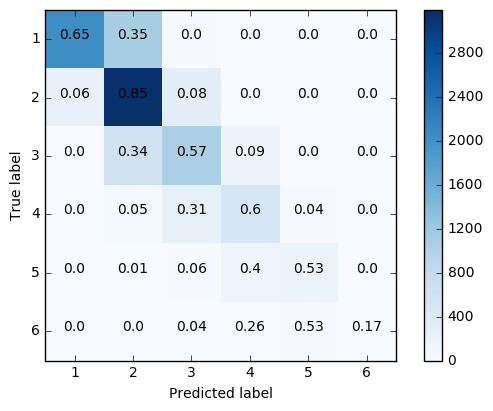
\includegraphics[width=.95\linewidth]{img/comb_d2_cm_retweets}
  \caption{Combined data set}
  \label{fig:retw_distr_sub4}
\end{subfigure}%
\caption{Confusion matrices for multi-input deep neural networks}
\label{fig:d2_cm}
\end{figure}

Once again, confusion matrices can deliver further insights into classification
performance.
Figures~\ref{fig:retw_distr_sub1} to~\ref{fig:retw_distr_sub3} show that up to
four out of six classes exhibit class accuracies above 50\% for the specialized
data sets.
Nevetheless, less common classes are still predicted poorly, in extreme cases
predictions are always incorrect here, e.g., for class six on politician and
company data.
It also becomes obvious that strong overall classification accuracy on company data
(73.52\%) is mainly based on high class accuracies for the most popular classes
1 and 2 (around 80\% accuracy).
Classification performance on the combined data set is more promising, as five
out of six classes are predicted with accuracies higher than 50\%.
Only the class with highest retweet counts is not predicted poorly, probably due
to the limited number of labeled examples stemming from this class.
Results on all data sets suggest that more training examples are
required for the model to generalize well to unseen data.
A possible indication about how many exampels are needed per class might be
given by class 2 of the combined data set, which shows a class accuracy of 85\%.
\outline{Add exact number of training examples for this class}
Further experiments could examine if similar performance can be achieved for
other classes, if the given number of examples are seen at training time.
All in all, classification are still biased towards more popular classes, where
the extent of the bias is dependent on overall data set size.
Another indication of biased behavior is the observation that misclassifications
on all data sets are pointed towards more popular classes.
For example, engagement is mainly underestimated on company and combined data set,
whereas overestimations occur for smaller classes of the celebrity data set.

\begin{table}
  \begin{tabular}{lrrrrrrr}
    \toprule
    & \multicolumn{7}{c}{Actual retweets} \\
    \midrule
    Data set & 0 & 1-10 & 10-100 & 100-1k & 1-10k & 10-100k & >100k \\
    \midrule
    Celebrities & 28.7 & 68.6 & 231.0 & 445.5 & 2,048.6 & 25,751.3 & 242,061.9 \\
    Politicians & 6.3 & 9.1 & 47.9 & 299.2 & 2,087.5 & 16,362.4 & - \\
    Companies & 0.5 & 3.2 & 17.8 & 185.4 & 2,099.5 & 13,939.7 & - \\
    Combined & 0.5 & 6.2 & 46.6 & 253.3 & 1,907.6 & 21,010.1 & 67,083.3 \\
    \bottomrule
    \toprule
    & \multicolumn{7}{c}{Actual favorites} \\
    \midrule
    Data set & 0 & 1-10 & 10-100 & 100-1k & 1-10k & 10-100k & >100k \\
    \midrule
    Celebrities & 10.1 & 27.4 & 339.2 & 795.4 & 2,047.8 & 23,117.3 & 161,387.5 \\
    Politicians & 30.2 & 20.5 & 70.7 & 267.2 & 2,056.0 & 18,204.5 & 108,637.6 \\
    Companies & 0.6 & 4.2 & 16.9 & 228.7 & 1,710.6 & 19,358.1 & - \\
    Combined & 1.0 & 6.5 & 46.5 & 403.8 & 1,878.7 & 18,932.1 & 89,079.0 \\
    \bottomrule
  \end{tabular}
  \caption[Detailed regression results for multi-input deep neural networks]{Mean absolute errors for specific ranges of actual engagement}
  \label{tab:d1_regression_eval}
\end{table}

\structure{Description of regression results}
\outline{Errors are still increasing with actual engagement}
\outline{Most imbalanced company data set shows lowest errors for many classes}
\outline{Zero values are predicted fairly well for company and combined data set}
\outline{Outliers have strong influence on mean calculation}
